\documentclass[10pt,a4paper]{scrartcl}
\usepackage[austrian]{babel}
\usepackage[utf8]{inputenc}
\usepackage{amssymb,amsmath} 
\usepackage{array}
\usepackage{subcaption}
\usepackage{graphicx} 
\usepackage{tikz}% for drawing automata etc 
\usetikzlibrary{automata,arrows,chains,shapes.misc,scopes,petri}
\usepackage{gslist}
\usepackage[counter-within=section]{exsheets}%http://www.ctan.org/pkg/exsheets
\SetupExSheets{counter-format=se.qu}
\SetupExSheets[solution]{print=true}
\DeclareTranslation{austrian}{exsheets-exercise-name}{Aufgabe}
\usepackage{enumitem}
\setlist[enumerate]{label=\alph*)}
\setlist[itemize]{label=--}
\newcommand{\vsp}{\vspace*{1cm}}


\newif\ifLoesung
\newcommand\Loesung[1]{\ifLoesung\begin{solution}#1\end{solution}\fi}



%: Einige Hilfsmakros
\newcommand\EA{{\mathcal{A}}}  % makro für das A für endliche Automaten
\newcommand\es{\varepsilon} % makro für Leerwort 
\newcommand{\ul}[1]{\underline{#1}} % für unterstreichen von einzelnen Symbolen einfach \ul x - wenn man ein Wort unterstrichen will \ul{wort}
\newcommand\sy[1]{{\underline{\ifmmode\mathtt{#1}\else\texttt{#1}\fi}}} % ähnlich wie \ul - verwendet aber andere Schriftart
\newlistt\sys\sy{\hspace{1pt}}{}{}{^} % identisch zu \sy, \sys{wort} unterstreicht aber jeden Buchstaben einzeln und \sy{wort} unterstreicht das ganze Wort 
% (sofern das Alphabet nur aus einzelnen Zeichen besteht ist \sys{wort} einfacher

% Korrekt ausfüllen
\newcommand\blatt{1}% Hier Blattnummer korrekt eintragen
\setcounter{section}{\blatt}
\Loesungtrue % Auskommentieren um Angabe zu kompilieren


\begin{document}
\begin{center}\LARGE\bfseries\sffamily
Theoretische Informatik und Logik\\
Übungsblatt \blatt ~ (2017W)
\ifLoesung\\Lösungen\fi
\end{center}
\medskip

Martin Szalay - 1526755


%:%%%%%%%%%%%%%%% BSP 1 %%%%%%%%%%%%%%%%%%%%%%%%%
\begin{question} Sei die Sprache $L$ gegeben durch folgende induktive Definition:
$L$ ist die kleinste Menge, sodass

\begin{itemize}
      \item $\sy \$\in L$
      \item $w\in L \Rightarrow xwx \in L$ f\"ur $x \in \{\sy a, \sy b\}$
\end{itemize}

(\textit{Anmerkung}: $L$ beschreibt Palindrome \"uber $\{\sy a, \sy b\}$, bei welchen das Symbol $\sy \$$ als Trennzeichen zwischen
einem Wort und seinem Spiegelbild fungiert.)

\begin{enumerate}
\item Geben Sie eine deterministische Turingmaschine $M$ an, welche die Sprache $L$ akzeptiert, und erl\"autern Sie (jeweils) 
auch kurz verbal die Arbeitsweise Ihrer Maschine. Es steht Ihnen dabei frei, ob Sie das auf Folie 26 definierte Modell 
(mit einem Band) oder das auf Folie 72 definierte Modell (mit zwei B\"andern, einem Eingabe- und einem Arbeitsband, wobei $M$ 
in diesem Fall die Kellerautomatenbedingung erf\"ullen soll) verwenden.  
 

\item Erweitern Sie Ihre unter a) gefundene Maschine so, dass sie $L'=\{w\sy \$w^r \mid w \in \Sigma^* \}$, 
wobei $\Sigma=\{\sy a_i \mid 1 \le i \le n\}$, akzeptiert. 
 
\end{enumerate}

\end{question}

\Loesung{% Your solution goes here
\begin{enumerate}
\item
\begin{tabular}{|c|c|c|c|c|c|}\hline
    $\delta$ & a & b & \$ & X & B \\ \hline
   q\textsubscript{0} & (q\textsubscript{0},a,R) & (q\textsubscript{0},b,R) & (q\textsubscript{1},\$,R) & (q\textsubscript{0},X,R) &  \\ \hline
   q\textsubscript{1} & (q\textsubscript{2},X,L) & (q\textsubscript{3},X,L) & (q\textsubscript{1},\$,L) & (q\textsubscript{1},X,L) & (q\textsubscript{4},B,R)  \\ \hline
   q\textsubscript{2} & (q\textsubscript{0},X,R) &  & (q\textsubscript{2},\$,L) & (q\textsubscript{2},X,L) &  \\ \hline
   q\textsubscript{3} &  & (q\textsubscript{0},X,R) & (q\textsubscript{1},\$,R) & (q\textsubscript{3},X,R) &  \\ \hline
   q\textsubscript{4} & & & & & (q\textsubscript{5},S,L)  \\ \hline
   q\textsubscript{5} & & & & &  \\ \hline
 \end{tabular}
\\
% M = ({qi | 0 <= i <= 5}, {a,b, \$}, {a,b,\$,X,B},  δ, q0, B, {q5})
$M = ( \big\{ q\textsubscript{i} 
\textbar 0 \le i \le 5 \big\} , \big\{ a,b,\$ \big\}, \big\{ a,b,\$, X, B \big\}, \delta, q\textsubscript{0}, B, \big\{q\textsubscript{5} \big\})$ \\

Idee:
Es wird das erste Symbol rechts vom Trennzeichen \$ und allen X genommen, danach wird in einen bestimmten Zustand gewechselt, welcher den aktuellen Buchstaben repraesentiert.\\
\\
q1 beliebiges Zeichen (a,b) darf eingelesen werden \\
q2 steht fuer a \\
q3 steht fuer b \\
X steht fuer "gelesen"\\
\\
Im Grunde faehrt die Maschine von rechts nach links bis diese ein Blank Symbol trifft, danach wird die andere Seite vom \$ angeschaut und haelt dann in q\textsubscript{5}.\\
Ein Blank Symbol kann nur beim einlesen nach rechts gefunden werden, sobald eines getroffen wird, haelt die Maschine.

\item 

$\delta$ =
$\big\{(q\textsubscript{0}, q\textsubscript{i}; q\textsubscript{0}, a\textsubscript{i}, R) \textbar 1 \le i \le n    \big\}         \rightarrow Istzustand, Folgezustand$ \\
$\cup \big\{(q\textsubscript{0}, \$; q\textsubscript{i}, \$, L) | 1 \le i \le n    \big\} $

$\cup \big\{(q\textsubscript{1}, \$; q\textsubscript{1}, \$, L), (q\textsubscript{1}, X; q\textsubscript{1}, X, L), (q\textsubscript{1}, B; q\textsubscript{n+2}, B, R),  \big\} \rightarrow zusammengefasst, weil i abhaengig$

$\cup \big\{(q\textsubscript{1}, a\textsubscript{i}; q\textsubscript{i+1}, X, R) | 1 \le i \le n    \big\}$ \\
$\cup \big\{q\textsubscript{i+1}, a\textsubscript{i};  q\textsubscript{1}, X, L) | 1 \le i \le n    \big\}$ \\
$\cup \big\{q\textsubscript{i+1}, \$;  q\textsubscript{i+1}, \$, R) | 1 \le i \le n    \big\}$ \\
$\cup \big\{q\textsubscript{i+1}, X;  q\textsubscript{i+1}, X, R) | 1 \le i \le n    \big\}$ \\

$\cup \big\{q\textsubscript{n+2}, \$;  q\textsubscript{n+2}, \$, R), \leftarrow vorletzter zustand, zus. weil n-abh.$ \\
$(q\textsubscript{n+2}, X;  q\textsubscript{n+2}, X, R), \leftarrow vorletzter zustand$ \\
$(q\textsubscript{n+2}, B;  q\textsubscript{n+3}, B, S), \leftarrow endzustand bei qn+3 
   \big\}$ \\

\end{enumerate}
}

%:%%%%%%%%%%%%%%% BSP 2 %%%%%%%%%%%%%%%%%%%%%%%%%
\begin{question} 

Seien $A$, $B$, $C$ und $D$ Sprachen, die rekursiv aufz\"ahlbar sein k\"onnen oder auch nicht.
Wir wissen allerdings Folgendes:

\begin{itemize}
  \item  $A \le B$
  \item  $B \le C$
  \item  $D \le C$
\end{itemize}


Geben Sie f\"ur jede der folgenden Aussagen an, ob sie
 
\begin{itemize}
  \item \textit{jedenfalls} zutrifft (unabh\"angig davon, um welche Probleme es sich bei $A$ bis $D$ handelt)
  \item \textit{vielleicht} zutrifft (je nach dem worum es sich bei $A$ bis $D$ handelt)
  \item \textit{keinesfalls} zutrifft (unabh\"angig davon, um welche Probleme es sich bei $A$ bis $D$ handelt)
\end{itemize}

Begr\"unden Sie jeweils Ihre Antwort.


\begin{enumerate}
  \item Ist $A$ entscheidbar, so ist auch das Komplement von $C$ entscheidbar.

  \item Ist das Komplement von $B$ nicht entscheidbar, so kann das Komplement von $C$ entscheidbar sein.

  \item Ist $C$ rekursiv aufz\"ahlbar, so ist auch $B \cup D$ rekursiv aufz\"ahlbar.

  \item Ist $A$ rekursiv aufz\"ahlbar, so ist $B$ entscheidbar.

  \item Ist $C$ nicht entscheidbar, so ist auch $D$ nicht entscheidbar.
\end{enumerate}

\end{question}

\Loesung{% Your solution goes here
\begin{enumerate}
\item
Jedenfalls, wenn C entscheidbar ist, so ist auch das Komplement entscheidbar. Da die Reduktion ist transitiv.
\item
Keinesfalls, wenn das Komplement von B nicht entscheidbar ist, so kann Komp von C auch nicht entscheidbar sein.
\item
Jedenfalls, da die Vereinigung von B und D auch eine Teilmenge von C ist.
\item
Vielleicht, aber nur wenn A entscheidbar ist.
\item
Vielleicht, da D entscheidbar sein koennte.

\end{enumerate}
}
%:%%%%%%%%%%%%%%% BSP 3 %%%%%%%%%%%%%%%%%%%%%%%%%
\begin{question}
Geben Sie an, ob folgende Probleme (un)entscheidbar sind, und begr\"unden Sie jeweils
Ihre Antwort. Sofern m\"oglich, verwenden Sie daf\"ur den \textit{Satz von Rice}.
(Das Alphabet ist dabei jeweils $\Sigma=\{\sy 0, \sy 1\}$.)

\begin{enumerate}
\item Gibt es f\"ur die von einer Turingmaschine akzeptierte Sprache genau eine Turingmaschine, die sie akzeptiert?
\item Ist die von einer Turingmaschine akzeptierte Sprache das Komplement von $\Sigma^*$?
\item Ist die Codierung der Turingmaschine, welche die Sprache $L$ akzeptiert, weniger als 1000 Symbole lang?
\item Ist das Komplement der von einer Turingmaschine akzeptierten Sprache endlich?
\item Ist die von einer Turingmaschine akzeptierte Sprache eine Teilmenge von $\Sigma^*$?
\end{enumerate}

\end{question}

\Loesung{
% Your solution goes here

\begin{enumerate}
\item
Entscheidbar, da es mindestens eine TM gibt. Satz von Rice nicht anwendbar.
\item
Entscheidbar, wenn das Komplement von $\Sigma^*$ L=\{\} ist. Laut Satz des Rice handelt es sich hierbei um eine triviale Eigenschaft.
\item
Unentscheidbar, da die TM nur dann akzeptiert wenn sie haelt. Sie koennte auch somit nicht halten.
\item
Unentscheidbar, da es nicht entscheidbar ist, ob eine Sprache endlich viele Woerter hat. 
zB L=\{\} Komplement von L = $\Sigma^*$ somit unendlich... nicht trivial
L=$\Sigma^+$ und das Komplement von L=\{$\epsilon$\} ... ist trivial
\item
Entscheidbar, da jede Sprache Woerter von $\Sigma^*$ enthaelt.

\end{enumerate}

}
%:%%%%%%%%%%%%%%% BSP 4 %%%%%%%%%%%%%%%%%%%%%%%%%
\begin{question} Sind folgende Aussagen korrekt? Begr\"unden Sie jeweils Ihre Antwort.

\begin{enumerate}
\item Ist $L_1$ regul\"ar, so ist auch $L_1 \cup L_2$ regul\"ar.

\item Ist $L_1\cap L_2$ entscheidbar, so sind $L_1$ und auch $L_2$ entscheidbar.

\item F\"ur jede rekursiv aufz\"ahlbare Sprache $L$ gilt: $L \cup \overline{L}$ ist entscheidbar.

\item Jedes unentscheidbare Problem enth\"alt eine entscheidbare Teilmenge.

\item Jede Teilmenge einer regul\"aren Sprache ist regul\"ar.
\end{enumerate}

\end{question}

\Loesung{
% Your solution goes here
\begin{enumerate}
\item
Falsch. Da man nicht weiss was $L_2$ ist. Es koennte nicht regulaer sein. Somit wir durch $L_1 \cup L_2$ die daraus resultierende Sprache auch nicht regulaer.

\item
Falsch. Es ware entscheidbar unter der Annahme dass sowohl $L_1$ als auch $L_2$ entscheidbar waren.

\item
Falsch.

\item
Falsch, da ein unentscheidbares Problem auch keine entscheidbaren Probleme enthalten kann.

\item
Richtig, da eine regulare Sprache aus kleinsten Teilmengen von regularen Sprachen besteht.

\end{enumerate}

}
%:%%%%%%%%%%%%%%% BSP 5 %%%%%%%%%%%%%%%%%%%%%%%%%
\begin{question} Sind folgende Sprachen regul\"ar? Falls ja, so geben Sie einen entsprechenden deterministischen 
endlichen Automaten an; falls nein, so beweisen Sie dies mit Hilfe des Pumping Lemmas f\"ur regul\"are Sprachen.
(W\"ahlen Sie mindestens zwei Unterpunkte.)

(\textit{Hinweis}: Nur eine der folgenden drei Sprachen ist regul\"ar.)
\begin{enumerate}

\item $\{u \sy \# v^r \mid u \mbox{ ist Bin\"ardarstellung (ohne f\"uhrende Nullen) von } n \mbox{, und } 
v \mbox{ jene von } n+1, n > 0 \} $. 

(W\"orter in dieser Sprache sind also z.B. $\sys{101\#011}$ und $\sys{1111\#00001}$)

\item Die Menge aller Bin\"arstrings (also W\"orter \"uber $\Sigma=\{\sy 0, \sy 1\}$), welche, interpretiert als Bin\"arzahl,
nicht durch 5 teilbar sind (ohne Ber\"ucksichtigung f\"uhrender Nullen).

\item $\{uu^ru  \mid u \in \{\sy a, \sy b, \sy c \}^*\}$
\end{enumerate}

(\textit{Hinweis}: $w^r$ bezeichnet das Spiegelbild von $w$.)

\end{question}

\Loesung{
% Your solution goes here


\begin{enumerate}
\item
Diese Sprache ist nicht regulaer. Beweis mit Pumping-Lemma: \\
\\
Wir waehlen ein Wort aus der Sprache, zB 1111\#00001 \\
Wir behaupten w=xyz, xy=1111 und z=\#00001\\
Dies erfuellt die Bedingungen vom Pumping-Lemma, da $|xy|\le$m und $|y|>0$\\
Laut Pumping-Lemma koennen wir schreiben: $w_i=xy^iz \in L$\\
\\
Wir suchen nun fuer y ein i, sodass es nicht mehr in der Sprache liegt.\\
\\
Probiere aus zB 2\\
Somit ware $w_i=xy^2z=a^{m+2} b^m$... Wir sehen sofort, dass es mehr als a als b gibt. Dies ist ein Widerspruch. Da das Wort nun wie folgt aussieht:\\
111111\#00001 .. links vom \# sind mehr Symbole als rechts.\\
...nicht regulaer.

\item
Diese Sprache ist regulaer. Beweis durch DEA

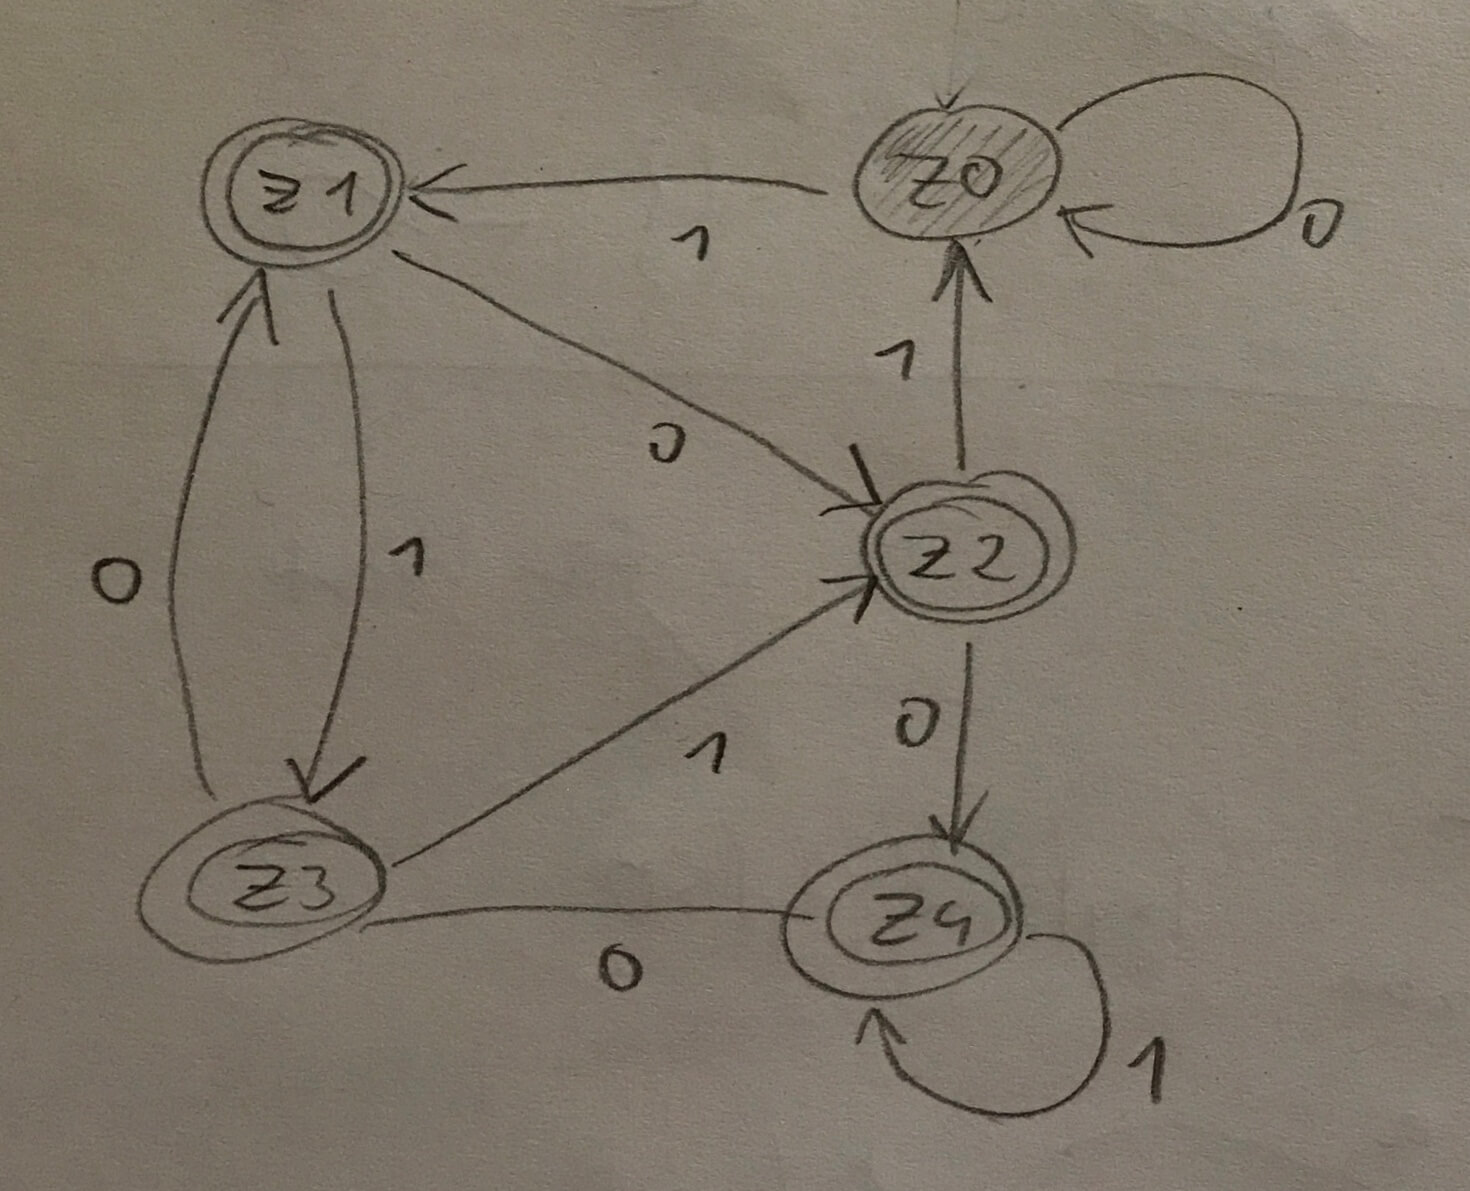
\includegraphics[width=0.7\textwidth]{DEA.JPG}

\item
Diese Sprache ist nicht regulaer. Beweis mit Pumping-Lemma:\\
\\
Wir waehlen ein Wort aus der Sprache, zB ab ba ab\\
Wir behaupten w=xyz, xy=ab und y=b\\
Pumping-Bedingung erfuellt, da $|xy|\le$m und $|y|>0$\\
Wir schreiben $w_i=xy^iz \in L$\\
\\
Wir suchen nun fuer y ein i, sodass es nicht mehr in der Sprache liegt.\\
\\
Probiere 4 aus.\\
Somit ware das Wort $ay^4baab$. Dies ist ein Widerspruch, da es sich $u^r$ kein Spiegelbild zum vorhergehenden u ist. Das Wort ware abbbbbaab.\\
$w=u^{m+4}u^ru^m$

\end{enumerate}



% Beispiel wie man mit Latex einen Automat zeichnet.
%
\begin{figure}[htb!]
% First subfigure
\begin{subfigure}[b]{0.50\textwidth}        \centering
\begin{tikzpicture}[->,>=stealth',shorten >=1pt,auto,node distance=1.7cm, thick,main node/.style={circle,fill=white,draw,font=\sffamily\bfseries}]

% Zustände definieren, initial für Startzustand, accepting für Endzustände
  \node[initial,accepting,state] (0) {0}; % in runder Klammer ist der Name den man anschließend verwendet um die Übergänge zu zeichnen, in geschwungenen Klammern ist die Beschriftung
  \node[state] (1) [below of=0] {1}; % below of = [Name von anderem Zustand] definiert die Position, es gibt: below of, right of, left of, above of, above right of, below right of
  \node[state] (2) [below of=1] {2};
  \node[state] (a) [right of=0]{a};
  \node[state] (b) [right of=1]{b};
  \node[state] (c) [right of=2]{c};
  \node[state] (x1) [right of=a]{x1};
  \node[state,accepting] (x2) [right of=c]{x2}; 
  
% Übergänge definieren 
  \path[every node/.style={font=\sffamily\small}]  % Falls man eine andere Schriftgröße, Liniendicke o.Ä. will kann man das hier anpassen
    (0) edge node {1}(1)  % (erster Zustand) edge node {Beschriftung} (zweiter Zustand)
    (1) edge node  {1} (2)
    (0) edge node[above]  {0} (a) % node[optionen] um anzugeben wo die Beschriftung hin soll (above, left, right, below)
    (1) edge node {0}(b)
    (2) edge[bend right] node{0}(c) % edge[bend left/ bend right] um gebogene Kante für Übergang zu verwenden
    (a) edge node[pos=0.2,left]{0}(x2) % pos=0.2 um festzulegen wo genau die Beschriftung ist (0 ist beim ersten Zustand, 1 beim zweiten)
    (c) edge node[pos=0.7,right]{0}(x1)
;
\end{tikzpicture}
\caption{Subcaption 1}\label{fig:ex}
\end{subfigure}
%
%
% Second subfigure
\begin{subfigure}[b]{0.50\textwidth}        \centering
\begin{tikzpicture}[->,>=stealth',shorten >=1pt,auto,node distance=1.8cm, thick,main node/.style={circle,fill=white,draw,font=\sffamily\bfseries}]
  \node[initial,accepting,state] (0) {0};
  \node[state,accepting] (1) [below of=0,node distance = 3.5cm] {1}; % falls man eine Distanz haben will die vom globalen Standard (hier als 1.8cm definiert) abweicht kann man das angeben
  \node[state] (m) [below right of=0]{m};
  \node[state] (0a) [above right of = m] {0a};
  \node[state] (1a) [below of=0a] {1a};
  \node[state,accepting] (2a) [below of =1a]{2a};
    \node[state] (0b)[right of = 0a]{0b};
      \node[state,accepting] (1b)[right of = 1a]{1b};
  \node[state] (2b)[right of = 2a]{2b};
  \node[state,accepting] (2c)[right of = 2b]{2c};
  
  \path[every node/.style={font=\sffamily\small}] 
   (0) edge node {1}(1)
    (0) edge node  {2} (m)
  (m) edge node[above]  {1} (0a)
  (0a) edge node {0}(1a)
  (0a) edge node{1}(0b)
  (1a) edge node{1}(2a)
   (0b) edge node{1}(1b)
   (1a) edge node{0}(1b)
   (0b) edge[bend left] node{0}(2b)
      (2b) edge node{0}(2c);
\end{tikzpicture}
\caption{Subcaption 2}\label{fig:mpl}
\end{subfigure}
\caption{EXaMPLe Automat}\label{fig:example}
\end{figure}
}
\end{document}
